\documentclass[tikz]{standalone}

\usepackage{xcolor}
\usepackage{tikz}
\usepackage{pgfplots}
\usepackage{amsmath}



% \newcommand{\midlinewidth}{0.6pt}
\newcommand{\midlinewidth}{1.0pt}
\newcommand{\largelinewidth}{1.7pt}
\newcommand{\middist}{17pt}
\newcommand{\largedist}{40pt}
\newcommand{\smalldist}{17pt}

\definecolor{lacamdarklilac5} {RGB} {51, 10, 102}
\colorlet{lacamdarklilac4} {lacamdarklilac5!80!}
\colorlet{lacamdarklilac3} {lacamdarklilac5!60!}
\colorlet{lacamdarklilac2} {lacamdarklilac5!40!}
\colorlet{lacamdarklilac1} {lacamdarklilac5!20!}

\definecolor{lacamgold5} {RGB} {255, 87, 0}
\colorlet{lacamgold4} {lacamgold5!80!}
\colorlet{lacamgold3} {lacamgold5!60!}
\colorlet{lacamgold2} {lacamgold5!40!}
\colorlet{lacamgold1} {lacamgold5!20!}
\definecolor{gold1} {RGB} {255, 180, 0}
\definecolor{violet} {RGB} {119, 111, 178}
\definecolor{petroil2} {RGB} {36, 165, 175}
\definecolor{petroil4} {RGB} {30, 132, 149}
\definecolor{petroil6} {RGB} {23, 101, 115}
\definecolor{gold2} {RGB} {255, 130, 0}
\definecolor{gold4} {RGB} {250, 100, 0}
\definecolor{gold6} {RGB} {245, 90, 0}

\definecolor{lacamoil5}{rgb}{0.13, 0.67, 0.8}
\colorlet{lacamoil4} {lacamoil5!80!}
\colorlet{lacamoil3} {lacamoil5!60!}
\colorlet{lacamoil2} {lacamoil5!40!}
\colorlet{lacamoil1} {lacamoil5!20!}

\usepackage{tikz}
\usetikzlibrary{circuits.logic.US}
\usetikzlibrary{shapes.misc}
\usetikzlibrary{shapes.arrows}
\usetikzlibrary{arrows,shapes.geometric}
\usetikzlibrary{patterns,calc,backgrounds}
\usetikzlibrary{trees}

\tikzstyle{nnf}=[
  >=latex, thick, >=stealth, font=\small,auto,scale=0.9,every node/.style={scale=0.9}
]
\tikzstyle{nnfnode}=[
  line width=1.0pt, draw
]
\tikzstyle{nnfand}=[
  nnfnode, and gate, rotate=90
]
\tikzstyle{nnfor}=[
  nnfnode, or gate, rotate=90
]
\tikzstyle{nnf2or}=[
  nnfor, inputs=nn
]
\tikzstyle{nnf2and}=[
  nnfand, inputs=nn
]
\tikzstyle{nnf3or}=[
  nnfor, inputs=nnn, scale=0.75
]
\tikzstyle{nnf4and}=[
  nnfand, inputs=nnnn, scale=0.65
]
\tikzstyle{nnfedge}=[
    line width=0.9
]
\tikzstyle{nnfterm}=[
  draw,fill=gray!10,inner sep=2.5pt, font=\small
]
\definecolor{hotcolor}{rgb}{0.85,0.0,0.0}
\tikzstyle{hot}=[
  draw=hotcolor, line width=1.1pt
]
\tikzstyle{hotparam}=[
  text=hotcolor
]

\begin{document}
% \begin{figure*}[t!]
% \begin{subfigure}[t]{0.17\textwidth}
% \centering
% \scalebox{.9}{
    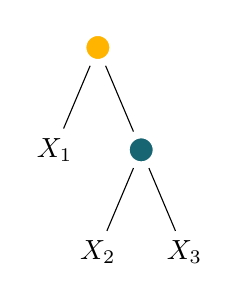
\begin{tikzpicture}[level distance=1.3cm,
      level 1/.style={sibling distance=1.1cm},
      level 2/.style={sibling distance=1.1cm}]
      \node[circle,fill=gold1,inner sep=4pt, line width=3pt, draw=white]{}
        child {node {$X_1$}     
        }
        child {node[circle,fill=petroil6,inner sep=4pt, line width=3pt, draw=white] {}
          child {node {$X_2$}}
          child {node {$X_3$}}
        };
    \end{tikzpicture}
% }
% \caption{A vtree}\label{fig: vtree}
% \end{subfigure}
% \begin{subfigure}[t]{0.37\textwidth}
% \centering
% \scalebox{0.67}{
    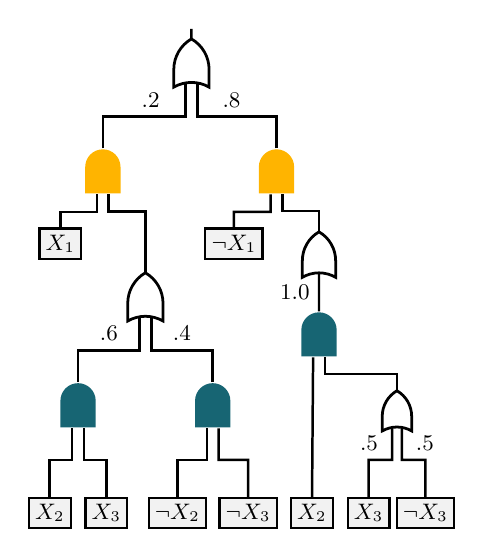
\begin{tikzpicture}[circuit logic US, nnf]
    \node (b1) [nnfterm]  at (0.0, 0.0) {$X_2$};
    \node (c1)  [nnfterm] at ($(b1) + (0.8, 0.0)$) {$X_3$};
    \node (not b)  [nnfterm]  at ($(c1) + (1.0, 0.0)$) {$\neg X_2$};
    \node (not c1) [nnfterm]  at ($(not b) + (1.0, 0.0)$) {$\neg X_3$};
    \node (b2)  [nnfterm] at ($(not c1) + (0.9, 0.0)$) {$X_2$};
    \node (c2)  [nnfterm] at ($(b2) + (0.8, 0.0)$) {$X_3$};
    \node (not c2)  [nnfterm] at ($(c2) + (0.8, 0.0)$) {$\neg X_3$};
    \node (or1) [nnf2or, scale=0.75] at ($(c2) + (0.4, 1.4)$) {};
    \node (and1) [nnf2and, scale=0.9,fill=petroil6, draw=none] at ($(b1) + (0.4, 1.5)$) {};
    \node (and2) [nnf2and, scale=0.9,fill=petroil6, draw=none] at ($(not b) + (0.5, 1.5)$) {};
    \node (and3) [nnf2and, scale=0.9,fill=petroil6, draw=none] at ($(b2) + (0.1, 2.5)$) {};
    \node (or2) [nnf2or, scale=0.9] at ($(and1) + (.95, 1.5)$) {\rotatebox{270}{}};
    \node (or3) [nnf3or, scale=0.9] at ($(and3) + (0.0, 1.1)$) {\rotatebox{270}{}};
    \node (a) [nnfterm] at ($(or2) + (-1.2, 0.8)$) {$X_1$};
    \node (not a) [nnfterm] at ($(or3) + (-1.2, 0.2)$) {$\neg X_1$};
    \node (and4) [nnf2and, scale=0.9,fill=gold1, draw=none] at ($(or2) + (-0.6, 1.8)$) {};
    \node (and5) [nnf2and, scale=0.9,fill=gold1, draw=none] at ($(or3) + (-0.6, 1.2)$) {};
    \node (root) [nnf2or, scale=0.9] at ($(and4) + (1.25, 1.5)$) {}; 
    \node (dummy) at ($(root) + (0.0, 0.4)$) {}; 
    \begin{scope}[on background layer]
    \draw [nnfedge] (c2) -- ++ (up:0.75) -| (or1.input 1)
        node[pos=0.4,above left] {$.5$};
    \draw [nnfedge] (not c2) -- ++ (up:0.75) -| (or1.input 2)
        node[pos=0.4,above right] {$.5$};
    \draw [nnfedge] (b1) -- ++ (up: 0.75) -| (and1.input 1);
    \draw [nnfedge] (c1) -- ++ (up: 0.75) -| (and1.input 2);
    \draw [nnfedge] (not b) -- ++ (up: 0.75) -| (and2.input 1);
    \draw [nnfedge] (not c1) -- ++ (up: 0.75) -| (and2.input 2);
    \draw [nnfedge] (b2) -- (and3.input 1);
    \draw [nnfedge] (or1.output) -- ++ (up: 0.22) -| (and3.input 2);
    \draw [nnfedge] (and1.output) -- ++ (up: 0.45) -| (or2.input 1)
         node[pos=0.4,above left] {$.6$};
    \draw [nnfedge] (and2.output) -- ++ (up: 0.45) -| (or2.input 2)
         node[pos=0.4,above right] {$.4$};
    \draw [nnfedge] (and3.output) -- (or3.input 2)
          node[pos=0.05,above left] {$1.0$};
    \draw [nnfedge] (a) -- ++ (up: 0.45) -| (and4.input 1);
    \draw [nnfedge] (or2.output) -- ++ (up: 0.85) -| (and4.input 2);
    \draw [nnfedge] (not a) -- ++ (up: 0.45) -| (and5.input 1);
    \draw [nnfedge] (or3.output) -- ++ (up: 0.28) -| (and5.input 2);
    \draw [nnfedge] (and4.output) -- ++ (up: 0.45) -| (root.input 1)
             node[pos=0.4,above left] {$.2$};
    \draw [nnfedge] (and5.output) -- ++ (up: 0.45) -| (root.input 2)
             node[pos=0.4,above right] {$.8$};
    \draw [nnfedge] (root.output) -- (dummy);
    \end{scope}
    \end{tikzpicture}
% }
% \caption{A PSDD}\label{fig:PSDD}
% \end{subfigure}
% \begin{subfigure}[t]{0.45\textwidth}
% \centering
% \scalebox{.65}{
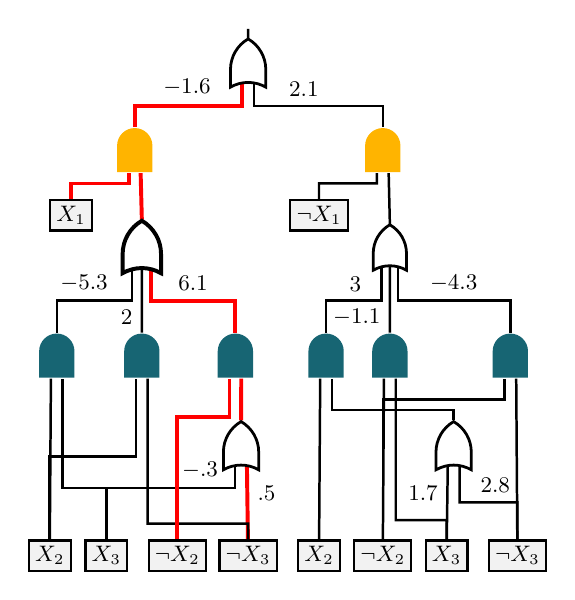
\begin{tikzpicture}[circuit logic US, nnf]
\node (b1) [nnfterm]  at (0.0, 0.0) {$X_2$};
\node (c1)  [nnfterm] at ($(b1) + (0.8, 0.0)$) {$X_3$};
\node (not b1)  [nnfterm]  at ($(c1) + (1.0, 0.0)$) {$\neg X_2$};
\node (not c1) [nnfterm]  at ($(not b1) + (1.0, 0.0)$) {$\neg X_3$};

\node (or1) [nnf2or, scale=0.9] at ($(not c1) + (-0.1, 1.5)$) {};
\node (and1) [nnf2and, scale=0.9,fill=petroil6, draw=none] at ($(b1) + (0.1, 2.8)$) {};
\node (and2) [nnf2and, scale=0.9,fill=petroil6, draw=none] at ($(c1) + (0.5, 2.8)$) {};
\node (and3) [nnf2and, scale=0.9,fill=petroil6, draw=none] at ($(or1) + (-0.08, 1.3)$) {};

\node (b2) [nnfterm]  at ($(not c1) + (1.0, 0.0)$) {$X_2$};
\node (not b2)  [nnfterm] at ($(b2) + (0.9, 0.0)$) {$\neg X_2$};
\node (c2)  [nnfterm]  at ($(not b2) + (0.9, 0.0)$) {$X_3$};
\node (not c2) [nnfterm]  at ($(c2) + (1.0, 0.0)$) {$\neg X_3$};

\node (or2) [nnf2or, scale=0.9] at ($(c2) + (0.1, 1.5)$) {};
\node (and4) [nnf2and, scale=0.9,fill=petroil6, draw=none] at ($(b2) + (0.1, 2.8)$) {};
\node (and5) [nnf2and, scale=0.9,fill=petroil6, draw=none] at ($(not b2) + (.1, 2.8)$) {};
\node (and6) [nnf2and, scale=0.9,fill=petroil6, draw=none] at ($(not c2) + (-0.1, 2.8)$) {};

\node (or3) [nnf3or, scale=0.9,line width=0.5mm] at ($(and2) + (0.0, 1.5)$) {};
\node (or4) [nnf3or, scale=0.9] at ($(and5) + (0.0, 1.5)$)
{};

\node (a) [nnfterm] at ($(or3) + (-1.0, 0.5)$) {$X_1$};
\node (not a) [nnfterm] at ($(or4) + (-1.0, 0.5)$) {$\neg X_1$};
\node (and7) [nnf2and, scale=0.9,fill=gold1, draw=none] at ($(or3) + (-.1, 1.4)$) {};
\node (and8) [nnf2and, scale=0.9,fill=gold1, draw=none] at ($(or4) + (-.1, 1.4)$) {};

\node (root) [nnf2or, scale=0.9] at ($(and7) + (1.6, 1.2)$)
{};
\node (dummy) at ($(root) + (0.0, 0.4)$) {};

\begin{scope}[on background layer]
\draw [nnfedge] (c1) -- ++ (up: 0.95) -| (or1.input 1)
    node[pos=0.47,above left] {$-.3$};
\draw [nnfedge, draw=red, line width=0.5mm] (not c1) -- (or1.input 2)
    node[pos=0.4,above right] {$.5$};
\draw [nnfedge] (b1) -- (and1.input 1);
\draw [nnfedge] (c1) -- ++ (up: 0.95) -| (and1.input 2);
\draw [nnfedge] (b1) -- ++ (up: 1.4) -| (and2.input 1);
\draw [nnfedge] (not c1) -- ++ (up: 0.45) -| (and2.input 2);
\draw [nnfedge, draw=red, line width=0.5mm] (not b1) -- ++ (up: 1.95) -| (and3.input 1);
\draw [nnfedge, draw=red, line width=0.5mm] (or1.output) -- (and3.input 2);
\draw [nnfedge] (c2) -- (or2.input 1)
    node[pos=0.4,above left] {$1.7$};
\draw [nnfedge] (not c2) -- ++ (up: .75) -| (or2.input 2)
    node[pos=0.4,above right] {$2.8$};
\draw [nnfedge] (b2) -- (and4.input 1);
\draw [nnfedge] (or2.output) -- ++ (up: 0.15) -| (and4.input 2);
\draw [nnfedge] (not b2) -- (and5.input 1);
\draw [nnfedge] (c2) -- ++ (up: .5) -| (and5.input 2);
\draw [nnfedge] (not b2) -- ++ (up: 2.2) -| (and6.input 1);
\draw [nnfedge] (not c2) -- (and6.input 2);
\draw [nnfedge] (and1.output) -- ++ (up: 0.45) -| (or3.input 1)
        node[pos=0.4, above left] {$-5.3$};
\draw [nnfedge] (and2.output) -- (or3.input 2)
        node[pos=0.5, below left] {$2$};
\draw [nnfedge, draw=red, line width=0.5mm] (and3.output) -- ++ (up: 0.45) -| (or3.input 3)
            node[pos=0.4,  above right] {$6.1$};
\draw [nnfedge] (and4.output) -- ++ (up: 0.45) -| (or4.input 1)
            node[pos=0.4, above left] {$3$};
\draw [nnfedge] (and5.output) -- (or4.input 2)
            node[pos=0.5, below left] {$-1.1$};
\draw [nnfedge] (and6.output) -- ++ (up: 0.45) -| (or4.input 3)
                node[pos=0.4,  above right] {$-4.3$};
\draw [nnfedge, draw=red, line width=0.5mm] (a) -- ++ (up: 0.45) -| (and7.input 1);
\draw [nnfedge, draw=red, line width=0.5mm] (or3.output) -- (and7.input 2);
\draw [nnfedge] (not a) -- ++ (up: 0.45) -| (and8.input 1);
\draw [nnfedge] (or4.output) -- (and8.input 2);
\draw [nnfedge, draw=red, line width=0.5mm] (and7.output) -- ++ (up: 0.3) -| (root.input 1)
    node[pos=0.4, above left] {$-1.6$};
\draw [nnfedge] (and8.output) -- ++ (up: 0.3) -| (root.input 2)
    node[pos=0.4, above right] {$2.1$};
\draw [nnfedge] (root.output) -- (dummy);
\end{scope}
\end{tikzpicture}

\end{document}

%%% Local Variables:
%%% mode: latex
%%% TeX-master: t
%%% End:


%%% Local Variables:
%%% mode: latex
%%% TeX-master: t
%%% End:
